\documentclass{article}
\usepackage[utf8]{inputenc}
\usepackage{textcomp}
\usepackage{booktabs,rotating,tabularx}
\usepackage{graphicx}
\usepackage[english]{babel}
\usepackage{caption}
\usepackage{float}
\usepackage{hyperref} % provides \url{}
\usepackage[shortlabels]{enumitem} % enumeration package
\usepackage[position=top]{subfig}
\usepackage{pdfpages}
\usepackage{listings}
\usepackage{tabularx}
\usepackage{float}

% page layout and margin
\usepackage[a4paper, margin=2.54cm]{geometry}

% list spacing
\usepackage{enumitem}
\setlist{topsep=2pt, itemsep=2pt, partopsep=2pt, parsep=2pt}
\def\arraystretch{1.5}
% Header & Footer
\usepackage{fancyhdr}
\pagestyle{fancy}
\lhead{Software Engineering 2 - DD}

\begin{document}

% title section
\begin{titlepage}
  \centering
  {\normalsize
    Software Engineering 2 - Prof. Camilli Matteo \\
    Dipartimento di Elettronica, Informazione e Bioingegneria \\
    Politecnico di Milano \par
  }     \vspace{3cm}
  {\Huge \textbf{CKB - CodeKataBattle\\} } \vspace{1cm}
  {\large \textbf{DD\\Design Document} \par} \vspace{1cm}
  {\normalsize January 7, 2024 \par} \vspace{4cm}
  {\normalsize Emanuele Pocelli (10726303) \\ Fabrizio Sordetti (10730069) \\  Andrea Varesi (10724377)\par} \vspace{4cm}
  \begin{figure}[h]
    \centering
    
\includegraphics[scale=0.3]{src/poli_logo.png}
  \end{figure} \vspace{0.5cm}
\end{titlepage}

\begin{large}
    
\tableofcontents

\section{Introduction}

\subsection{Purpose}

The system has, as main function, to deliver a platform where Students can challenge themselves, alone or in team, writing code to solve exercises assigned by Educators, to improve their software development skills. Students have to follow a test-first approach.
\\The platform is used by Educators to create, manage and close tournaments, each one is composed by battles, while Students have to solve the exercises published for every battle filling them with their own code. Each exercise includes a brief textual description and a software project with build automation scripts that contains a set of test cases that the program must pass, but without the program implementation.
\\CKB offres also the possibility for each team to know their rank (calculated automatically by the platform) within the context of each battle, and the general rank of that tournament, in addition to a set of badges the Students can achieve, to increase the level of challenge. 

\vspace{24pt}

\subsection{Scope}

The CodeKataBattle system is designed with the primary objective of providing a comprehensive platform for students to hone their programming skills through the collaborative resolution of coding exercises. The system follows the principles of \textit{codekata}, emphasizing the iterative practice of problem-solving for effective learning. \\In addition to catering to students, the system accommodates a second user category: educators. Educators are empowered to oversee various aspects of the tournaments they create, wielding a range of functionalities. This includes the creation of battles, the assignment of problems to students, and the evaluation of the projects submitted by participants. \\Each battle within the system is defined by specific deadlines, imposing a structured timeline on student endeavors. Participants are required to diligently work on their projects, ensuring compliance with the technical specifications set for their respective workspaces. Furthermore, the platform extends its utility by offering features such as the visualization of tournament and battle ranks, as well as the opportunity for students to earn badges upon completion of a tournament. \\For a more detailed exploration of these features, refer to the Requirements Analysis and Specification Document (RASD).

\newpage

\subsection{Definitions, Acronyms, Abbreviations}

\subsubsection{Definitions}

\begin{itemize}
    \item \textbf{Programming language}: set of rules that allows string values to be converted into various ways of generating machine code, or, in the case of visual programming languages, graphical elements.
    \item \textbf{Automation scripts}: a specific type of automation script used in software development to automate the process of building, compiling, and packaging software applications.
    \item \textbf{Test-first approach}: is a software development process relying on software requirements being converted to test cases before software is fully developed, and tracking all software development by repeatedly testing the software against all test cases.
    \item \textbf{GitHub}: a platform and cloud-based service for software development and version control, allowing developers to store and manage their code.
    \item \textbf{Badge}: elements in the form of rewards that represent the achievements of individual students.
    \item \textbf{ACID properties}: (atomicity, consistency, isolation, durability) is a set of properties of database transactions intended to guarantee data validity despite errors, power failures, and other mishaps.
\end{itemize}

\vspace{12pt}

\subsubsection{Acronyms}

\begin{itemize}
    \item \textbf{CKB}: CodeKataBattle
    \item \textbf{RASD}: Requirement Analysis and Specification Document 
    \item \textbf{DD}: Design Document
    \item \textbf{UML}: Unified Modelling Language
    \item \textbf{UI}: User Interface
    item \textbf{REST}: Representational state transfer
    \item \textbf{DBMS} - database management system
    \item \textbf{API} - Application Programming Interface
    \item \textbf{ER} - entity-relationship
    \item \textbf{HTTP} - hypertext transfer protocol
    \item \textbf{SPA} - Single Page Application
    \item \textbf{JSON} - JavaScript Object Notation
    \item \textbf{XML} - eXtensible Markup Language
\end{itemize}

\vspace{12pt}

\subsubsection{Abbreviations}

\begin{itemize}
    \item $[Rn]$ - the n-th functional requirement
    \item $[Fn]$ - the n-th feature 
    \item S2B - software to be
\end{itemize}

\vspace{24pt}

\subsection{Revision History}

\begin{itemize}
    \item Version 1.0 (07/01/2024)
\end{itemize}

\vspace{1cm}

\subsection{Reference Documents}

This document is based on: 
\begin{itemize}
    \item The specification of the RASD and DD assignment of the Software Engineering II course, held by professor Matteo Rossi, Elisabetta Di Nitto and Matteo Camilli at the Politecnico di Milano, A.Y 2023/2024
    \item Slides of Software Engineering 2 course on WeBeep;
    \item Official link of Codewars (https://www.codewars.com/), a platform similar to CodeKataBattle
    \item Other information that helped the development of the project: 
    \begin{itemize}
        \item In-depth analysis on \href{http://codekata.com/}{codekata};
        \item In-depth analysis on \href{https://en.wikipedia.org/wiki/Test-driven\textunderscore development}{test-driven development};
    \end{itemize}
\end{itemize}

\vspace{24pt}

\subsection{Document Structure}

This document is divided in 6 chapters, more in detail:

\begin{itemize}
    \item \textbf{Introduction}: this chapter explains what are the purpose and the scope of the project, adding some technical information such as definitions and acronyms of terms used in the document and references.
    \item \textbf{Architectural Design}: it introduces the main architectural choices made for the system. This section includes an overview of the components and interfaces to communicate, a description of the infrastructure and also diagrams to represent both static and runtime views.  
    \item \textbf{User Interface Design}: this chapter contains the mock-ups both for educator and student interfaces, including a brief description of the main functionalities provided by the interface. 
    \item \textbf{Requirement Traceability}: this section shows the links between requirements (previously defined in RASD) and components described in the previous chapters.
    \item \textbf{Implementation, Integration and Test Plan}: this chapter describes the correct order to deploy the system, starting from the subsystems and components implementation, then integrating and testing.   
    \item \textbf{Effort spent}: this section shows the time spent (in hours) by each member to work on this document.
    \item \textbf{References}: it contains the references to any documents and to the Software used in this document.
\end{itemize}

\section{Architectural Design}

The purpose of this section is to present and analyze the architecture of the software to be system in a top-down manner. We first introduced the overall architecture and then provided a diagram of the system’s components, focusing on the tournaments and battles sub-components. Next, we used an ER diagram to describe the system’s logical data and presented the system’s deployment view, including the layers and tiers involved. We also used sequence diagrams to depict important runtime views and class diagrams to analyze the component interfaces. Finally, we discussed the architectural design choices and the reasons behind them.

\subsection{Overview}
The figure shown below represents a high-level description of the components which make up the System.
It is a distributed system with a 4-tier architecture: presentation, web server, application server and database. In this document, the presentation layer and the Client will be referred to as the Frontend, while the Application Layer and the Data Layer will be referred to as the Backend.
\\
\begin{figure}[h]
    \center
    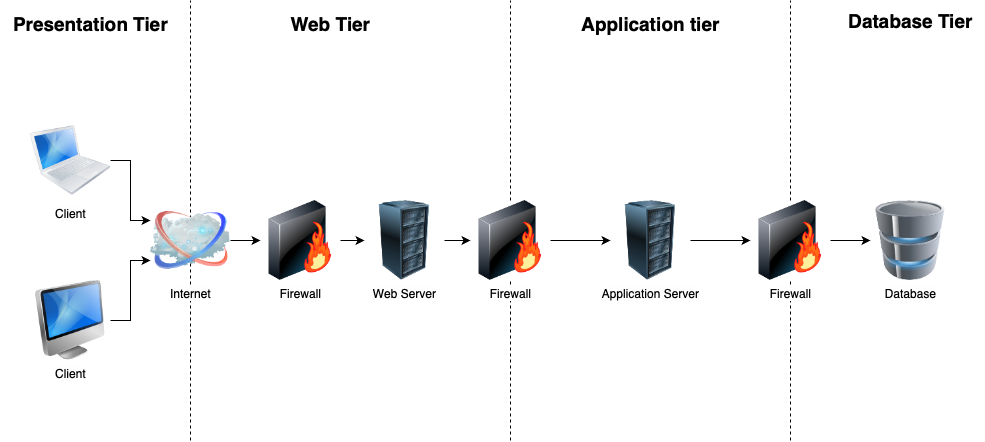
\includegraphics[width=1\linewidth]{src/High level system architecture.png}
    \caption{High level system architecture}
    \label{fig:High level system architecture}
\end{figure}
\\
The presentation tier is the client side, where users interact with the system through a web browser. A single page application will be developed both for educators and students to use the system. The reason behind this choice is the ease of interaction without the need for frequent page reloading, providing a better user experience.\\
The web server is responsible for communication between the Frontend and the Backend. It handles HTTP requests, routing them to the appropriate components. It supports secure communication with clients through HTTPS, and load balancing ensures optimal performance during periods of high traffic.\\
The application tier is the logic core of our system. It processes data received from the presentation tier, performs business logic operations, and communicates with the database. It tier ensures data integrity, security, and authentication, with role-based access controls. It interfaces with external services or APIs as needed. \\
Finally, the data tier is responsible for storing, reading and updating all information necessary for the system. We use a relational database that offers high scalability potential for structured data.
It interfaces with the application tier, granting data access and manipulation while respecting security protocols.\\
The client web-server and web-server application-server communication use HTTP, while app-server DBMS communication relies on APIs. The app-servers are designed to be stateless according to REST standards. The system also includes firewalls to enhance security.\\

\subsection{Component view}
In this section we offer a more detailed view of the S2B. We will focus on the components and their interactions, along with the interfaces. To meet performance and availability criteria, most of said components will be duplicated or replicated.
\begin{figure}[h]
    \centering
    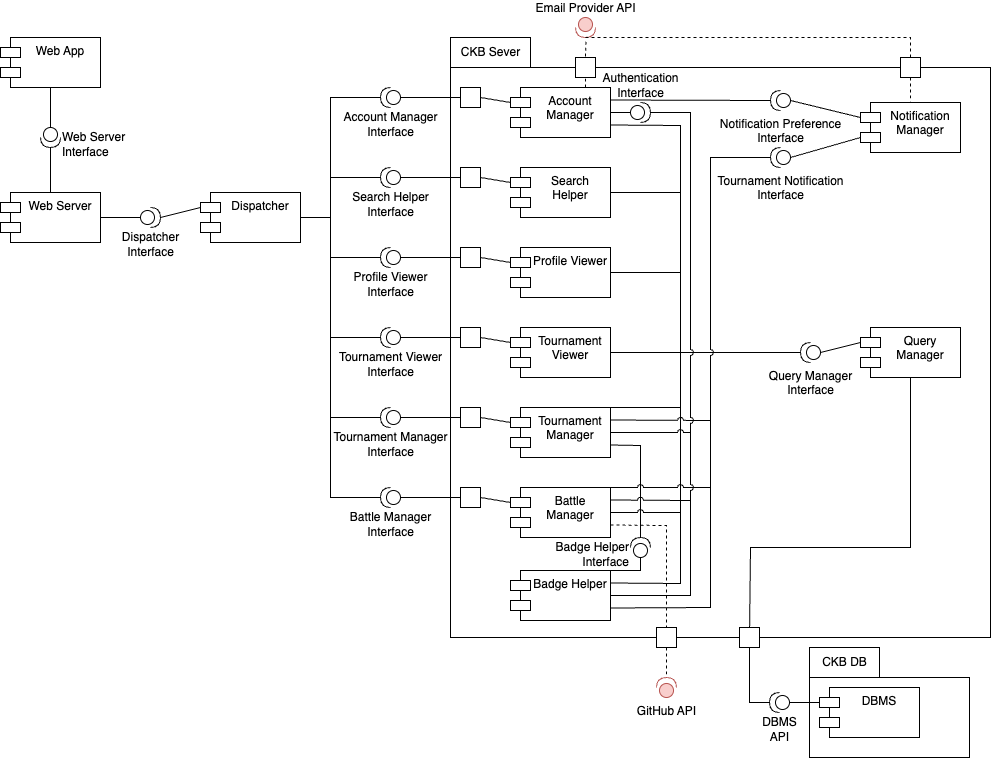
\includegraphics[width=1\linewidth]{src/Component Diagram of the CKB System.png}
    \caption{Component Diagram of the CKB System}
    \label{fig:Component Diagram of the CKB System}
\end{figure}
\\
\\
\\
\begin{itemize}
    \item \textbf{Web server}\\
    The web server is designed to handle HTTP requests from the client, redirecting them to the appropriate components. It uses client-side rendering. As the user interacts with the page, further requests may be automatically made and the page will be updated dynamically without requiring a full page reload.\\
    \item \textbf{CKB server}\\
    The CKB server is responsible for the business logic and provide the full functionality to users. Since most of the functionalities offered are shared between educators and students, there will not be a different server for each user category. It is further composed of different components.\\
    \begin{itemize}
        \item \textbf{CKB’s Account Manager}\\
        This component handles all the account operations related to the users and offers an interface to authenticate the requests. It offers functionality to create new account, logging in, setting preferences and verify the authentication of the user at any time. To create a new account, It interacts with the external email provider API to make the user receive a code to verify the identity.\\
        \item \textbf{Search helper}\\
        This component enables the search functionality, letting users and non-users search for a specific user or a specific tournament. It also allows filtering based on date posted, number of awards, ongoing/finished, number of participants and much more (tournaments).\\
        \item \textbf{Profile viewer}\\
        This component allows viewing profiles of users subscribed to CKB, both educators and students. Anyone can see profiles, even unsubscribed users. Within the profile page, there may be tournaments the user took part in (as a student or as an educator) and clicking them will redirect that tournament page.\\
        \item \textbf{Tournament viewer}\\
        This component allows viewing tournaments, along with the battle pages in the scope of It. Anyone can see tournaments, even unsubscribed users. You can find all the information related to that tournament, as well as the battles, including teams, final rank for each battle and much more.\\
        \item \textbf{Tournament manager}\\
        This component allows managing and creating tournaments for educators and subscribing to them for students. The creator can grant other educators permission to create battles. For ongoing tournaments, allowed educators can create new battle clicking the right button. Such functionality is provided through the next component.\\
        \item \textbf{Battle manager}\\
        This component allows managing and creating battles for educators and joining them for students. It also manages the team functionality, allowing students to team up for each battle. \\
        \item \textbf{Badge helper}\\
        This component enables the gamification aspects of CKB. It allows educators to create badges and define new rules as well as new variables associated with them. Badges are then linked to the profile of users achieving them, making them visible to anyone.\\
        \item \textbf{CKB Notification Service}\\
        This component enables the CKB notifications. Users will receive notifications about important events, like new tournaments created, tournament to which the user is subscribed closes and more.
        \newline
        \newline
        \textbf{External APIs}\\
        \item \textbf{GitHub API}\\
        This API enables the GitHub integration: new repositories automatically created (e.g. when a new battle begins) and sources automatically downloaded (e.g. when a user pushes new code to the main branch of his repository)\\
        \item \textbf{Email provider API}
        This service is used for authentication during registration and for important notifications.
    \end{itemize}
    \vspace{1cm}
    \item \textbf{Query Manager}
    \\This component is responsible for communicating with the Database Management System. It follows the adapter pattern, allowing  easier communication between other components and the DBMS.
\end{itemize}

\vspace{1cm}

\subsection{Deployment view}
This chapter describes the deployment of the system.
\begin{figure}[h]
    \centering
    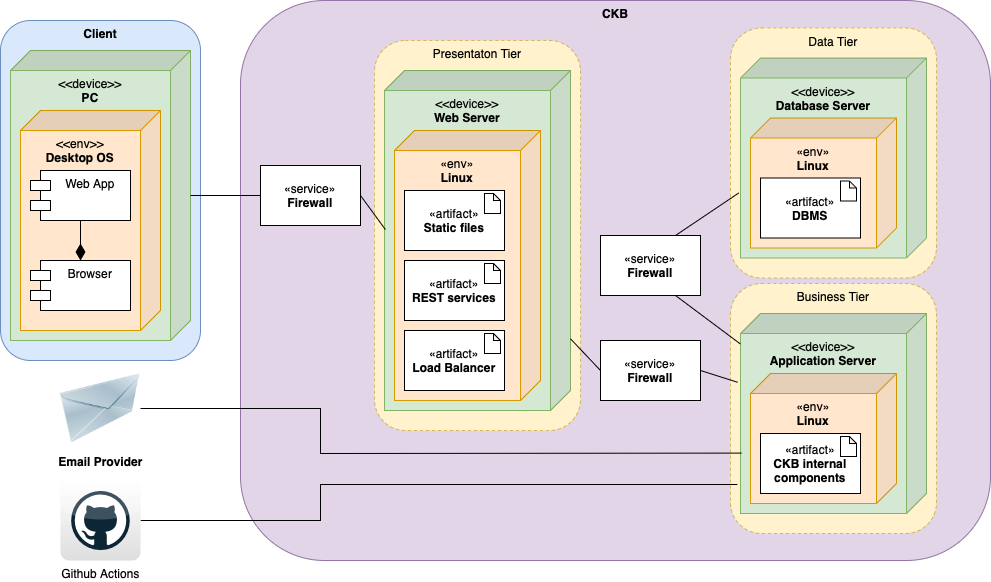
\includegraphics[width=1\linewidth]{src/Deployment View of the system.png}
    \caption{Deployment View of the system}
    \label{fig:Deployment View of the system}
\end{figure}
\\
\begin{itemize}
    \item \textbf{Web-server}\\
    The web-server will be the entry point for the SPA. It forwards the requests to the application-server. A modern device with access to a web browser is required to interface with the web-server. 
    \item \textbf{Load Balancer}\\
    This device is responsible for load balancing, which means, distributing incoming network traffic and requests across multiple servers. Its primary purpose is to optimise resource utilization, enhance reliability while ensuring high availability.
    \item \textbf{Firewall}\\
    Firewalls are used to filter connections to the application and data layers of a system. They are located between the internet and the system intranet. They offer additional security blocking or allowing traffic based on predetermined rules.
\end{itemize}

\subsection{Runtime View}
This section illustrates the interactions between actors, subsystems and interfaces of the system showing the specific method called.

\subsection{Component Interfaces}
This section lists all the methods offered by each component interface to the other components.

\subsection{Selected architectural styles and patterns}
\begin{itemize}
    \item \textbf{Three layer four tier}\\
    This architecture offers several benefits. It allows the distinction of layers (presentation, logic, data) and tiers (client, web server, application server, DBMS), which makes the system more modular and easier to maintain. Such separation also allows better scalability and better workload distribution across multiple servers. Finally, load balancing and caching techniques are available to further increase performance and availability.

    \item \textbf{RESTful APIs}\\
    The API is based on standard web technologies, like JSON or XML, allowing better integration with other systems. It is stateless, which makes the development easier. It also promotes simplicity and scalability.\\
    \item \textbf{Adapter pattern}\\
    The Adapter Pattern seamlessly integrates different components, standardizing interfaces and ensuring flexibility. It hides the underlying complexity and provides a set of high-level functions. 
\end{itemize}

\vspace{1cm}
    
\subsection{Other design decisions}
\begin{itemize}
    \item SQL database
    SQL databases offer high scalability and decent performance for structured data. It follows ACID principles and ensures data integrity. Overall, It is a good compromise for performance, consistency, reliability and ease of use.
\end{itemize}
\section{User Interface Design}

\begin{figure}[h]
    \centering
    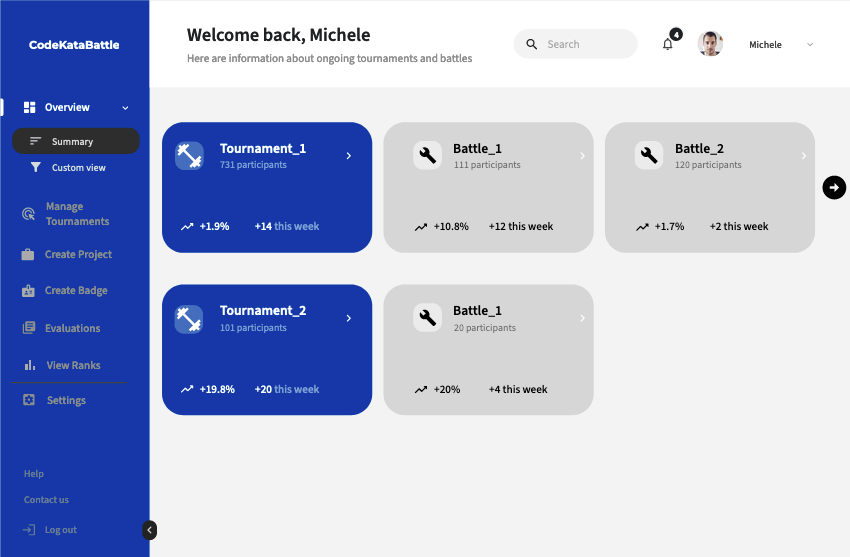
\includegraphics[scale=0.5]{src/educator_view.png}
    \caption*{Educator Interface}
\end{figure} \vspace{0.5cm}

In the Educator Interface the main page shows the ongoing tournaments, followed by every ongoing battle for that tournament. \\The search bar allows educator to search for a nickname and find users associated to it, so that it's possible to visualize their profile. \\The main functions an educator can perform are shown on the left column: 
\begin{itemize}
    \item \textbf{Manage Tournaments}: allows an educator to create and close a tournament, create (with all the possible settings) and close battles and eventually grant the permission to create battles to another educator.
    \item \textbf{Create Project}: allows an educator to create a new project to assign to students. 
    \item \textbf{Create Badge}: allows an educator to create a new badge that could be achieved by the students in a tournament.
    \item \textbf{Evaluations}: allows an educator to manually evaluate students' projects.
    \item \textbf{View Ranks}: view all ongoing tournaments and battles rank.
\end{itemize}

\vspace{100pt}

\begin{figure}[H]
    \centering
    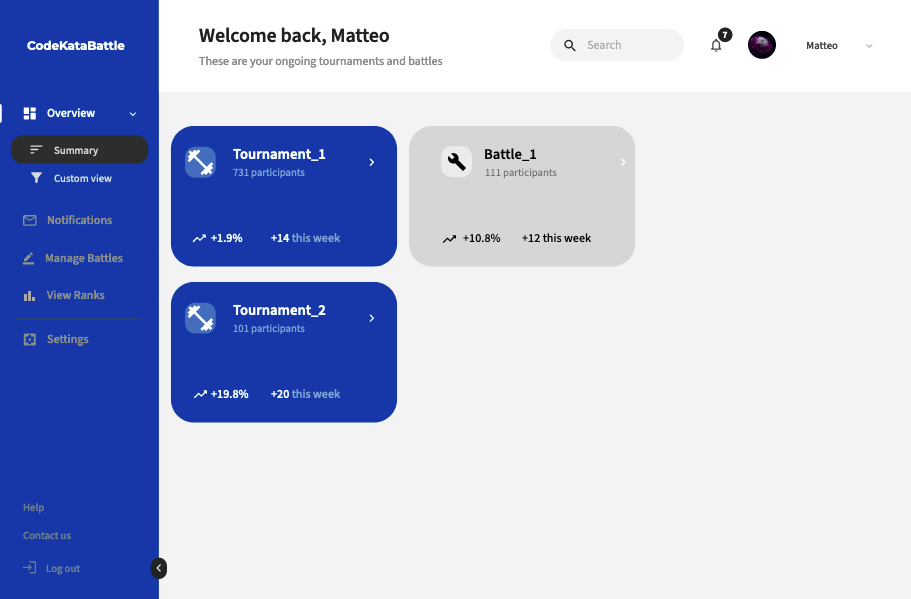
\includegraphics[scale=0.45]{src/student_view.png}
    \caption*{Student Interface}
\end{figure} \vspace{0.5cm}

In the Student Interface the main page shows the ongoing tournaments, followed by the battles to which the student is subscribed. \\The search bar allows student to search for a nickname and find users associated to it, so that it's possible to visualize their profile. \\The main functions a student can perform are shown on the left column:
\begin{itemize}
    \item \textbf{Notifications}: allows a student to view the notifications the platform sends when a new tournament or a new battle within a tournament the student is subscribed to is created.
    \item \textbf{Manage Battles}: this section allows a student to create teams and contains the link to the GitHub repository for each battles he/she is subscribed to. 
    \item \textbf{View Ranks}: view all ongoing tournaments and battles rank.
\end{itemize}

\section{Requirement Traceability}

This section aims to map each requirement previously defined in the RASD document to the design elements that compose the CKB system and that satisfy it.

\vspace{1cm}

\begin{table}[H]
  \centering
  \begin{tabularx}{\textwidth}{|p{3cm}|X|}
    \hline
    \textbf{Requirements:} &
    $[R1]$: The system allows educators to sign up
    \newline$[R2]$: The system allows students to sign up
    \\
    \hline
    \textbf{Components:} & 
    \begin{itemize}
        \item Web App
        \item Web Server
        \item Dispatcher 
        \item CKB Server 
        \begin{itemize}
            \item CKB's Account Manager 
        \end{itemize}
        \item Query Manager
        \item DBMS
        \item Email Provider API
    \end{itemize}
    \\
    \hline
  \end{tabularx}
\end{table}


\begin{table}[H]
  \centering
  \begin{tabularx}{\textwidth}{|p{3cm}|X|}
    \hline
    \textbf{Requirements:} &
    $[R3]$: The system allows registered educators to log in
    \newline$[R4]$: The system allows registered students to log in
    \\
    \hline
    \textbf{Components:} & 
    \begin{itemize}
        \item Web App
        \item Web Server
        \item Dispatcher 
        \item CKB Server 
        \begin{itemize}
            \item CKB's Account Manager 
        \end{itemize}
        \item Query Manager
        \item DBMS
    \end{itemize}
    \\
    \hline
  \end{tabularx}
\end{table}


\begin{table}[H]
  \centering
  \begin{tabularx}{\textwidth}{|p{3cm}|X|}
    \hline
    \textbf{Requirements:} &
    $[R5]$: The system allows educators to create a new tournament
    \newline$[R6]$: The system allows an educator to grant permission to create battles within the context of a specific tournament to another educator
    \newline$[R24]$ The system allows educators who created a tournament to close it
    \\
    \hline
    \textbf{Components:} & 
    \begin{itemize}
        \item Web App
        \item Web Server 
        \item Dispatcher
        \item CKB Server 
        \begin{itemize}
            \item CKB's Account Manager
            \item Tournament Manager 
        \end{itemize}
        \item Query Manager
        \item DBMS
    \end{itemize}
    \\
    \hline
  \end{tabularx}
\end{table}


\begin{table}[H]
  \centering
  \begin{tabularx}{\textwidth}{|p{3cm}|X|}
    \hline
    \textbf{Requirements:} &
    $[R7]$: The system allows educators to create a new battle, if they have the permission to do it
    \\
    \hline
    \textbf{Components:} & 
    \begin{itemize}
        \item Web App
        \item Web Server 
        \item Dispatcher 
        \item CKB Server 
        \begin{itemize}
            \item CKB's Account Manager
            \item Tournament Manager
            \item Battle Manager 
        \end{itemize}
        \item Query Manager
        \item DBMS
    \end{itemize}
    \\
    \hline
  \end{tabularx}
\end{table}


\begin{table}[H]
  \centering
  \begin{tabularx}{\textwidth}{|p{3cm}|X|}
    \hline
    \textbf{Requirements:} &
    $[R8]$: The system notifies all the students subscribed to the platform when a new tournament is created
    \\
    \hline
    \textbf{Components:} & 
    \begin{itemize}
        \item Web App
        \item Web Server
        \item Dispatcher 
        \item CKB Server 
        \begin{itemize}
            \item Tournament Manager
            \item CKB Notification Service 
        \end{itemize}
        \item Query Manager
        \item DBMS
    \end{itemize}
    \\
    \hline
  \end{tabularx}
\end{table}



\begin{table}[H]
  \centering
  \begin{tabularx}{\textwidth}{|p{3cm}|X|}
    \hline
    \textbf{Requirements:} &
    $[R9]$: The system allows students to subscribe to a tournament
    \\
    \hline
    \textbf{Components:} & 
    \begin{itemize}
        \item Web App
        \item Web Server 
        \item Dispatcher
        \item CKB Server 
        \begin{itemize}
            \item CKB's Account Manager
            \item Search Helper
            \item Tournament Manager 
        \end{itemize}
        \item Query Manager
        \item DBMS
    \end{itemize}
    \\
    \hline
  \end{tabularx}
\end{table}


\begin{table}[H]
  \centering
  \begin{tabularx}{\textwidth}{|p{3cm}|X|}
    \hline
    \textbf{Requirements:} &
    $[R10]$: The system notifies all the students subscribed to a specific tournament when a new battle in the context of that tournament is created 
    \\
    \hline
    \textbf{Components:} & 
    \begin{itemize}
        \item Web App
        \item Web Server 
        \item Dispatcher
        \item CKB Server 
        \begin{itemize}
            \item Battle Manager 
            \item CKB Notification Service
        \end{itemize}
        \item Query Manager 
        \item DBMS
    \end{itemize}
    \\
    \hline
  \end{tabularx}
\end{table}



\begin{table}[H]
  \centering
  \begin{tabularx}{\textwidth}{|p{3cm}|X|}
    \hline
    \textbf{Requirements:} &
    $[R11]$: The system allows educators that created a battle to upload the code kata
    \newline$[R12]$ The system allows educators that created a battle to set minimum and maximum number of students per group
    \newline$[R13]$ The system allows educators that created a battle to set a registration deadline
    \newline$[R14]$ The system allows educators that created a battle to set a final submission deadline
    \newline$[R15]$ The system allows educators that created a battle to set the possibility to manually evaluate projects during the consolidation stage
    \newline$[R16]$ The system allows students to create teams for ongoing battles inviting other students 
    \newline$[R17]$ The system allows students to join a battle
    \newline$[R20]$ The system allows educators to manually evaluate projects during the consolidation stage in the context of a specific battle 
    \\
    \hline
    \textbf{Components:} & 
    \begin{itemize}
        \item Web App
        \item Web Server 
        \item Dispatcher
        \item CKB Server 
        \begin{itemize}
            \item CKB's Account Manager
            \item Battle Manager 
        \end{itemize}
        \item Query Manager 
        \item DBMS
    \end{itemize}
    \\
    \hline
  \end{tabularx}
\end{table}


\begin{table}[H]
  \centering
  \begin{tabularx}{\textwidth}{|p{3cm}|X|}
    \hline
    \textbf{Requirements:} &
    $[R18]$: The system sends to each student that belongs to a team subscribed to a battle the link of the GitHub repository assigned to that team
    \\
    \hline
    \textbf{Components:} & 
    \begin{itemize}
        \item Web App
        \item Web Server 
        \item Dispatcher
        \item CKB Server 
        \begin{itemize}
            \item Battle Manager 
            \item CKB Notification Service
        \end{itemize}
        \item GitHub API
        \item Query Manager 
        \item DBMS
    \end{itemize}
    \\
    \hline
  \end{tabularx}
\end{table}



\begin{table}[H]
  \centering
  \begin{tabularx}{\textwidth}{|p{3cm}|X|}
    \hline
    \textbf{Requirements:} &
    $[R19]$: The system allows both students and educators to see the current rank evolving during a battle 
    \newline$[R22]$ The system allows both educators and students to see the list of ongoing tournaments
    \newline$[R23]$ The system allows both educators and students to see the rank of each ongoing tournament
    \\
    \hline
    \textbf{Components:} & 
    \begin{itemize}
        \item Web App
        \item Web Server 
        \item Dispatcher
        \item CKB Server 
        \begin{itemize}
            \item Tournament Viewer
        \end{itemize}
        \item Query Manager 
        \item DBMS
    \end{itemize}
    \\
    \hline
  \end{tabularx}
\end{table}



\begin{table}[H]
  \centering
  \begin{tabularx}{\textwidth}{|p{3cm}|X|}
    \hline
    \textbf{Requirements:} &
    $[R21]$ The system notifies all students participating in the battle when the final battle rank becomes available 
    \newline$[R25]$ The system notifies all students involved in a tournament when the final rank of that tournament becomes available
    \\
    \hline
    \textbf{Components:} & 
    \begin{itemize}
        \item Web App
        \item Web Server 
        \item Dispatcher
        \item CKB Server 
        \begin{itemize}
            \item Tournament Viewer
            \item CKB Notification Service
        \end{itemize}
        \item Query Manager 
        \item DBMS
    \end{itemize}
    \\
    \hline
  \end{tabularx}
\end{table}


\begin{table}[H]
  \centering
  \begin{tabularx}{\textwidth}{|p{3cm}|X|}
    \hline
    \textbf{Requirements:} &
    $[R26]$ The system allows educators that have created a tournament to create badges 
    \\
    \hline
    \textbf{Components:} & 
    \begin{itemize}
        \item Web App
        \item Web Server 
        \item Dispatcher
        \item CKB Server 
        \begin{itemize}
            \item CKB's Account Manager
            \item Tournament Manager
            \item Badge Helper 
        \end{itemize}
        \item Query Manager 
        \item DBMS
    \end{itemize}
    \\
    \hline
  \end{tabularx}
\end{table}


\begin{table}[H]
  \centering
  \begin{tabularx}{\textwidth}{|p{3cm}|X|}
    \hline
    \textbf{Requirements:} &
    $[R27]$ The system allows both educator and students to visualize the profile and badges of a student 
    \\
    \hline
    \textbf{Components:} & 
    \begin{itemize}
        \item Web App
        \item Web Server 
        \item Dispatcher
        \item CKB Server 
        \begin{itemize}
            \item Profile viewer
        \end{itemize}
        \item Query Manager 
        \item DBMS
    \end{itemize}
    \\
    \hline
  \end{tabularx}
\end{table}

\section{Implementation, Integration and Test Plan}

\subsection{Overview}

The aim of this chapter is to show how to implement the system, then how to integrate the various components with each other and finally how to plan the test phases, in order to offer simplifications during the development of the whole system.
\\First, there is a description about how to implement, integrate and test single components. After that, the second step consists in defining the methods to follow to test the whole system and last there are some concerns about additional information regarding the testing process.

\subsection{Implementation, Component Integration and Testing Plan}

Here is a summary regarding the components that together constitute the CKB system:

\vspace{0.5cm}

\begin{itemize}
    \item \textbf{Web Server}
    \item \textbf{CKB Server}
    \begin{itemize}
        \item \textbf{CKB's Account Manager}
        \item \textbf{Search Helper}
        \item \textbf{Profile Viewer}
        \item \textbf{Tournament Viewer}
        \item \textbf{Tournament Manager}
        \item \textbf{Battle Manager}
        \item \textbf{Badge Helper}
        \item \textbf{CKB Notification Service}
    \end{itemize}
    \item External components
    \begin{itemize}
        \item \textbf{Github API}
        \item \textbf{Email Provider API}
    \end{itemize}
    \item \textbf{Query Manager}
\end{itemize}

\vspace{0.5cm}

To implement the system, we decided to opt for a bottom-up approach. By focusing on individual components and building gradually, it yields a more modular and scalable design. This facilitates specific modifications without impacting the entire system. 
\\Moreover, it promotes adaptability and flexibility, enabling optimization of distinct parts without compromising the overall technical project.
\\To follow the bottom-up approach, we highlighted the difficulty level to implement each component and we also provided a development order based on the dependencies between each component with the others, leading to a decision about the sequence of steps of implementation, component integration and testing. 
\\In the following steps we assume that DBMS component is already implemented and available (it is not represented for simplicity), to focus on the main components and sub-components of CKB system. 

\begin{table}[H]
    \centering
    \begin{tabular}{|c|c|}
        \hline
        Order & Stage\\
        \hline
        0 &
        $[F0]$ DB Interaction\\
        \hline
        1 & 
        $[F1]$ User Notifications\\
        \hline
        2 & 
        $[F2]$ Create Account and Log in\\
        \hline
        3 & 
        $[F3]$ View Profiles\\
        \hline
        4 &
        $[F4]$ Search Features\\
        \hline
        5 &
        $[F5]$ Managing Battles\\
        \hline
        6 & 
        $[F6]$ Managing Tournaments\\
        \hline
        7 &
        $[F7]$ Tournaments and Battles Features\\
        \hline
    \end{tabular}
    \caption*{Features Identification - Server Side}
\end{table}

\vspace{1cm}

\subsection{Development Stages Definition}

Here is a description about the steps to follow to implement, integrate and test the components of the system following the features enumeration described above.
\\Each component uses a driver to simulate other components not already implemented.

\begin{enumerate}
    \vspace{1cm}
    \item \textbf{DB Interaction}: the first component that must be implemented in the system is Query Manager, that offers to almost all other components in CKB server an interface to communicate indirectly with the DBMS.
    \vspace{0.5cm}
    \begin{figure}[H]
        \centering
        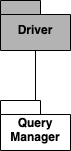
\includegraphics[scale=0.6]{src/phase0.drawio.png}
    \end{figure} 
    \vspace{0.5cm}
    \newpage
    \item \textbf{User Notifications}: this is the second step of the implementation and integration of components that satisfy the requirements for the CKB system. In this phase it's introduced and tested the Notification Manager to handle the notifications that the system sends to users. It offers interfaces to other components that will later be developed.
    \vspace{0.5cm}
    \begin{figure}[H]
        \centering
        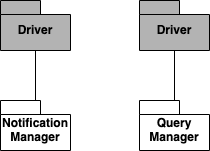
\includegraphics[scale=0.6]{src/phase1.drawio.png}
    \end{figure} 
    \vspace{2cm}
    \item \textbf{Create Account and Log in}: than component that have to be implemented is the one who manage the basic features to access the systems, that is creating a new account or logging in, with all the features that result from it, such as setting preferences or verifying an account whenever needed.
    The component that manages these features is CKB's Account Manager, the third one to be implemented and for which the unit tests have to be provided.
    Account Manager is integrated with Notification Manager as it leverages functionalities exposed by that component and with Query Manager to interact with DBMS.
    \vspace{0.5cm}
    \begin{figure}[H]
        \centering
        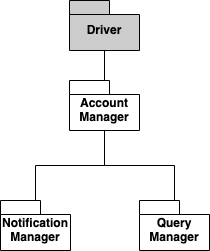
\includegraphics[scale=0.6]{src/phase2.drawio.png}
    \end{figure} 
    \vspace{0.5cm}
    \newpage
    \item \textbf{View Profiles}: the next phase consists in implementing and test Profile Viewer component, the one that manages user's profiles. It is integrated with Query Manager as it interacts with the DBMS to accomplish its operations.
    \vspace{0.5cm}
    \begin{figure}[H]
        \centering
        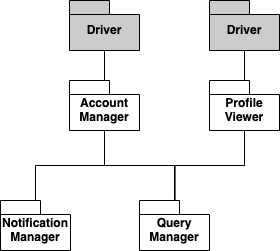
\includegraphics[scale=0.6]{src/phase3.drawio.png}
    \end{figure} 
    \vspace{2cm}
    \item \textbf{Search Features}: the next component that has to be implemented and tested is Search Helper. It offers the possibility to search for user profiles and to search for a tournament with filtering options.  It is integrated with Query Manager as it interacts with the DBMS to accomplish its operations.
    \vspace{0.5cm}
    \begin{figure}[H]
        \centering
        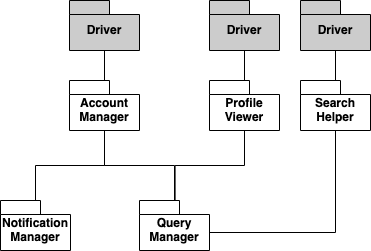
\includegraphics[scale=0.6]{src/phase4.drawio.png}
    \end{figure} 
    \vspace{0.5cm}
    \newpage
    \item \textbf{Managing Battles}: in this step must be implemented one of the core components for the system, Battle Manager. It offers an interface for the following component and it interacts with Account Manager so these two components have to be integrated.  It is integrated also with Query Manager as it interacts with the DBMS to accomplish its operations.
    \vspace{0.5cm}
    \begin{figure}[H]
        \centering
        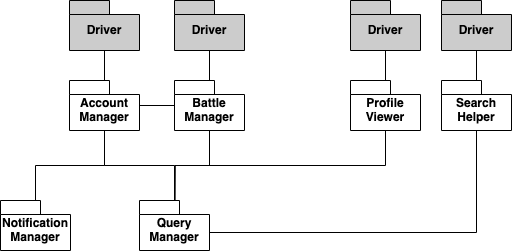
\includegraphics[scale=0.6]{src/phase5.drawio.png}
    \end{figure} 
    \vspace{0.5cm}
    \item \textbf{Managing Tournaments}: this is one of the most important feature of the system and the component that fulfill it is Tournament Manager, that offers all the features described previously in this document. Moreover, due to the possibility for educators to create badges before a tournament, in this phase is implemented also the Badge Helper component. Both components are integrated with Account Manager because many operations require the profile authentication to be executed. For both of these components must be provided the appropriate unit tests. The Tournament Manager component is also integrated with Battle Manager and Notification Manager to fulfill the main operations regarding the life cycle of a tournament. Finally, the component is integrated with Query Manager to interact with DBMS.
    \vspace{0.5cm}
    \begin{figure}[H]
        \centering
        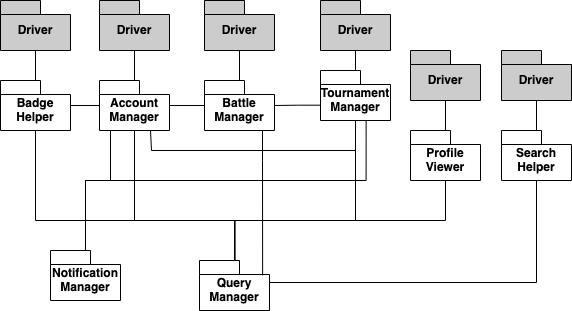
\includegraphics[scale=0.6]{src/phase6.drawio.png}
    \end{figure} 
    \vspace{0.5cm}
    \newpage
    \item \textbf{Tournaments and Battles Features}: this step implements and integrates in the system the Tournament Viewer component. It is integrated with Query Manager as it interacts with the DBMS to accomplish its operations.
    \vspace{0.5cm}
    \begin{figure}[H]
        \centering
        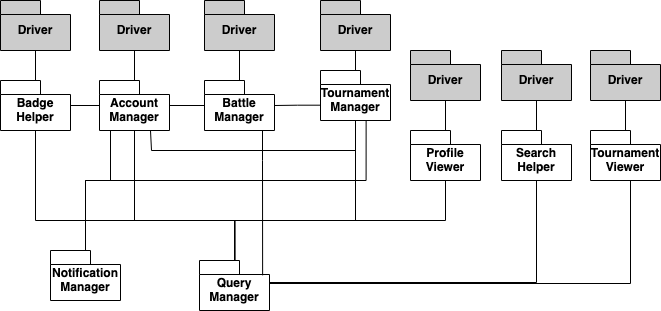
\includegraphics[scale=0.6]{src/phase7.drawio.png}
    \end{figure} 
    \vspace{0.5cm}
    \item \textbf{Dispatcher}: this component has to be implemented and tested to allow the correct interaction with different components.
    It's integrated with almost all the components previously described, so this phase is crucial to build and develop a working system. 
    \vspace{0.5cm}
    \begin{figure}[H]
        \centering
        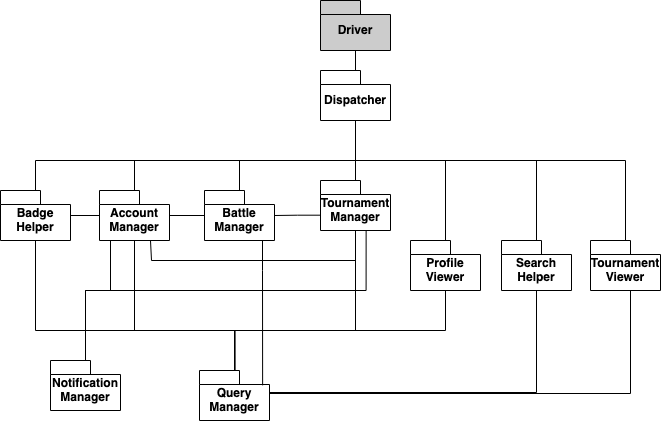
\includegraphics[scale=0.6]{src/phase8.drawio.png}
    \end{figure} 
    \vspace{0.5cm}
    \newpage
    From now on are implemented components to allow the communication between the client-side and the server-side.
    \vspace{2cm}
    \item \textbf{Web Server}: this component interacts from the server-side with the Dispatcher, so when the Web Server is implemented and tested, it has to be integrated with it.
    \vspace{0.5cm}
    \begin{figure}[H]
        \centering
        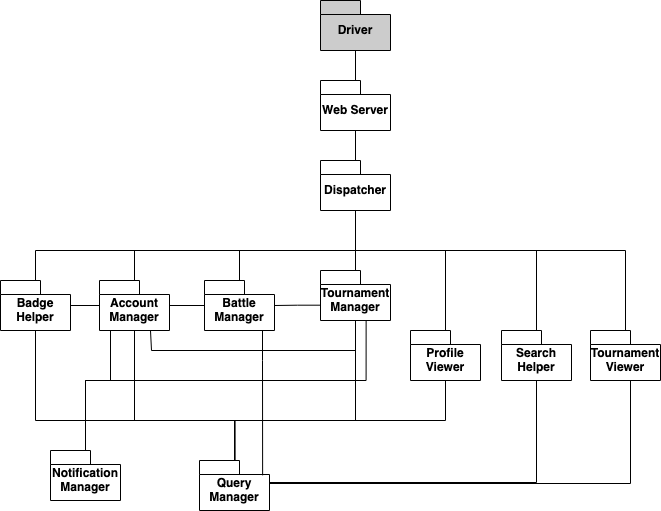
\includegraphics[scale=0.6]{src/phase9.drawio.png}
    \end{figure} 
    \vspace{0.5cm}
    \newpage
    \item \textbf{Web App}: this component represents the system on the client-side. It offers an interface to communicate with the server-side (it has to be integrated with Web Server). This interaction must be carefully curated down to the smallest details as it represents the main interaction between users and system.
    \vspace{0.5cm}
    \begin{figure}[H]
        \centering
        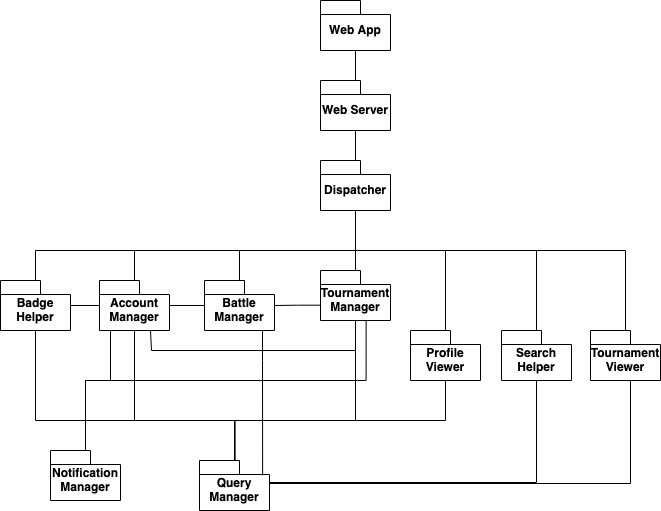
\includegraphics[scale=0.6]{src/phase10.drawio.png}
    \end{figure} 
    \vspace{0.5cm}
\end{enumerate}

\vspace{1cm}

\subsection{System testing}
\vspace{0.5cm}
This phase consider the system as a whole and concerns the testing of all the functionalities that the system has to fulfill, analyzing the requirements defined in the RASD. 
\\System testing is a more complicated step with respect to unit testing, and has to be performed by developers but with also an interaction with stakeholders, to make sure that the system is as close as possible to the desired final product.
\\
\\Different system testing techniques can be adopted and executed:
\begin{itemize}
    \item \textbf{Functional testing}: to check whether to software meets the requirements.
    \item \textbf{Performance Testing}: to highlight bottlenecks and measure response time and throughput and also hardware and network issues. To do so the testers have to load the system with expected workload and compare performances.
    \item \textbf{Load Testing}: to highlight bugs concerning the memory usage. To do so the testers have to load the system with increasing workload and for a long period.
    \item \textbf{Stress Testing}: to make sure that the system recovers gracefully after failure. The testers have to try to break the system under test by overwhelming its resources or by reducing resources.
\end{itemize}

\vspace{1cm}

\subsection{Additional specifications on testing}
A key point that must be underlined is that this is only a first version of the CKB system, so whenever new functionalities or changes in the requirements are made, the developers must check as first thing the functionalities added, and then also executing integration tests and system tests that can find new bugs before releasing a new version of the system. 
\\Once more, during the whole process, is important having an interactions with the stakeholders to take right decisions to create the right product.

\section{Effort Spent}


\begin{table}[h]
  \centering
  \caption*{Emanuele Pocelli}
  \begin{tabularx}{\textwidth}{|X|X|}
    \hline
    \textbf{Chapter} & \textbf{Effort (in hours)}\\
    \hline
    1 & 1\\
    \hline
    2 & 25\\ 
    \hline
    3 & 2\\
    \hline 
    4 & 2\\ 
    \hline
    5 & 2\\
    \hline
  \end{tabularx}
\end{table}

\begin{table}[h]
  \centering
  \caption*{Fabrizio Sordetti}
  \begin{tabularx}{\textwidth}{|X|X|}
    \hline
    \textbf{Chapter} & \textbf{Effort (in hours)}\\
    \hline
    1 & 1\\
    \hline
    2 & 25\\
    \hline
    3 & 1\\
    \hline 
    4 & 3\\
    \hline
    5 & 3\\
    \hline
  \end{tabularx}
\end{table}

\begin{table}[h]
  \centering
  \caption*{Andrea Varesi}
  \begin{tabularx}{\textwidth}{|X|X|}
    \hline
    \textbf{Chapter} & \textbf{Effort (in hours)}\\
    \hline
    1 & 3\\
    \hline
    2 & 3\\
    \hline
    3 & 5\\
    \hline 
    4 & 6\\
    \hline
    5 & 15\\
    \hline
  \end{tabularx}
\end{table}

\section{References}

\begin{itemize}
    \item Diagrams made with: \href{https://app.diagrams.net}{draw.io}
    \item Mockups made with: \href{https://moqups.com/it/}{moqups.com}
    \item Testing models and component architecture made with: \href{https://app.diagrams.net}{draw.io}
    \item High level architectures are made with: \href{https://app.diagrams.net}{draw.io}
\end{itemize}


\end{large}

\end{document}